%Para hacer informe con portada utilizamos report

\documentclass[12pt,oneside]{book}

\usepackage[a4paper]{geometry}
\usepackage[myheadings]{fullpage}
\usepackage{fancyhdr}
\usepackage{lastpage}
\usepackage{graphicx, wrapfig, subcaption, setspace, booktabs}
\usepackage[T1]{fontenc}
\usepackage[font=small, labelfont=bf]{caption}
\usepackage{fourier}
\usepackage[protrusion=true, expansion=true]{microtype}

%Paquete para hipervinculos
\usepackage[colorlinks=true]{hyperref}
\hypersetup{
    colorlinks=true,
    linkcolor=black,
    filecolor=magenta,      
    urlcolor=blue,
}

%Para qué los subtítulos aparezcan en español
\usepackage[spanish]{babel}
\usepackage[utf8]{inputenc}
\usepackage{sectsty}
\usepackage{url, lipsum}
\usepackage{tabularx}
\usepackage{float}

%--------------------------------------------------
%Para agregar citas en apa
%Para citar se usa el comando \cite{}
%Las referencias se modifican en el archivo sample.bib
\usepackage{apacite}
%----------------------------------------------

\newcommand{\HRule}[1]{\rule{\linewidth}{#1}}
\onehalfspacing
\setcounter{tocdepth}{5}
\setcounter{secnumdepth}{5}

%-------------------------------------------------------


\begin{document}


%-------------------------------------------------------------------------------
% Portada
%-------------------------------------------------------------------------------
\begin{titlepage}
    \begin{center}
        \vspace*{1cm}
            
        \Huge
        \textbf{La memoria del computador}
            
        \vspace{0.5cm}
        \LARGE
        
            
        \vspace{1.5cm}
            
        \textbf{Geraldine Ramirez Londoño }
            
        \vfill
            
        \vspace{0.8cm}
            
        \Large
        Despartamento de Ingeniería Electrónica y Telecomunicaciones\\
        Universidad de Antioquia\\
        Medellín\\
        Septiembre de 2020
            
    \end{center}
\end{titlepage}
\newpage

\tableofcontents
%-------------------------------------------------------
\newpage
\section{Introducción}


En el presente documento se abordara el tema de la memoria del computador y los diferentes tipos existentes de esta, entre los cuales podemos encontrar la memoria HDD o disco duro, SDD, RAM y memoria cache, entre otras. Con la respectiva explicación de su funcionalidad, y caracteristicas de cada memoria, adicionalmente se mencionara la forma en que estas ayudan al correcto funcionamiento del computador. 

\section{La memoria del computador }
Es importante iniciar definiendo la palabra memoria, donde es un término genérico usado para designar las partes del computador o de los dispositivos periféricos donde todos los datos y programas son almacenados. \cite{memoria-computadora}

Entonces podríamos decir que la memoria  es uno de los componentes fundamentales para que todo funcione correctamente en nuestro PC, ya que su existencia permite que el computador pueda arrancar, se procesen los datos, se puedan ejecutar las instrucciones para los distintos programas y demás. De acuerdo a lo anterior vamos a continuar mencionando los diferentes tipos de memoria y su funcionalidad


\section{Tipos de memoria}
Un computador trabaja como minimo con cuatro tipos de memoria diferentes, y cada una de ellas se encarga de realizar una función distinta. Estas son la memoria RAM, memoria ROM, la memoria SRAM o Caché, HDD o disco duro, entre otras.

 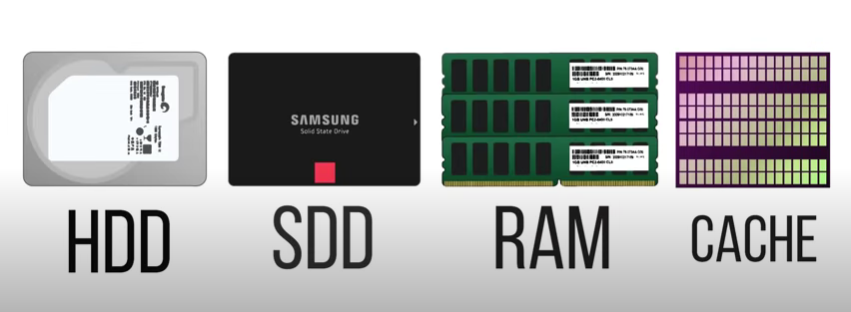
\includegraphics[width=1.00\textwidth]{MEMORIAS.PNG}
  La imagen corresponde al video de  \cite{memoria}
 \newpage
 
 \begin{itemize}
        \item { Memoria HHD (disco duro o unidad de estado solido )}:
        
        Siendo uno de los componentes mas importante de cualquier sistema informatico. El disco duro es un dispositivo de almacenamiento de datos en el cual podemos guardar cualquier tipo de información digital. Ya sean fotografías, vídeos, archivos de texto o programas informáticos.
        
        En cuanto a su funcionamiento este tiene varios discos internos y cada vez que se solicita un archivo debe buscarlo dentro de estos discos, tiene una tabla donde esta apuntado  el sitio de cada uno de estos archivos, el cual se llama “Sistema de ficheros “  y  luego procede a buscar los datos en la posición indicada.
        
         \item { Memoria SSD (unidad de estado sólido)}:
         
         Cumple con la función de almacenar datos de tu ordenador. Básicamente, un SSD hace lo mismo que un HDD, La gran diferencia es que mientras los discos duros utilizan componentes mecánicos que se mueven, las SSD almacenan los archivos en microchips con memorias flash interconectadas entre sí.
        
         \item { Memoria RAM (memoria principal) }:
         
         La memoria RAM, es el área de trabajo del ordenador y en ella se encuentran tanto las instrucciones  como los datos que está utilizando el procesador o el CPU del ordenador para trabajar en el momento.
         
         En otras palabras, es un tipo de memoria que nos permite almacenar temporalmente información a una velocidad elevada, haciendo que el dispositivo informático  funcione y realice tareas automatizadas. Estos datos se pierden cuando el equipo ya sea una computadora, portátil, Smartphone o tableta se apaga.  
         
         La memoria RAM siendo la memoria principal del computador ha venido cambiando y  mejorando a medida que pasan los años. Entre los tipos de memoria RAM más conocidos podemos encontrar:
         
        \begin{itemize}
            \item Memoria SDRAM: Este tipo de memoria RAM es muy simple de identificar porque tiene dos muescas de separación entre contactos. Estos contactos son 168 en total y puede trabajar a velocidades de 66 y 133MHz. En la actualidad se encuentran en desuso.
            \item Memoria DDR: Estas memorias son las sucesoras de las SDRAM y poseen sólo una muesca de separación. Además cuentan con 184 contactos y su velocidad de trabajo es superior, ya que se encuentra entre 200 y 600 MHz. Tienen la particularidad de realizar dos intercambios de datos por un ciclo de reloj.
            \item Memoria DDR2: La evolución natural de la memoria DDR. Se diferencia de las anteriores por que posee 240 contactos y la velocidad de trabajo va desde 400 hasta 800 MHz. Por demás está decir se comercializan en pares de 2GB cada una.
            \item Memoria DDR3: Son la tercera generación de memorias DDR. Posee casi las mismas características de la DDR2, pero su velocidad de trabajo puede duplicar y hasta triplicar la versión anterior. En la actualidad es el tipo de memoria RAM más utilizada.
            \item Rambus: Es un tipo de memoria especial que posee 184 contactos y velocidades que van desde 600 hasta 1066 MHz. Son costosas ya que cuentan con disipadores de calor incluidos. 
            \item So-DIMM: Similares al Rambus pero mucho más pequeñas y son utilizadas en equipos portátiles. Cuentan con diferentes tipos según el número de contactos y velocidad de trabajo.
            
            la definicion de los tipos de memoria RAM corresponde a.\cite{RAM}
        
        \end{itemize}

        
         \item { Memoria SRAM (memoria cache)}:
         
         La memoria cache es el área de almacenamiento dedicada a los datos usados o solicitados con más frecuencia, para su recuperación a gran velocidad. Podemos decir que es un intermediario entre la RAM y la memoria del procesador.
        
         \item { Memoria VRAM (memoria de la tarjeta gráfica)}:
         
        La tarjeta de vídeo o tarjeta gráfica se encarga de procesar los datos que le llegan del procesador para generar una salida que podrá representarse en un monitor.
        
        Es un tipo de memoria específicamente diseñada para su uso en soluciones gráficas, y juega un papel muy similar al de la RAM principal, aunque obviamente dentro de su propio campo.
        
        Según donde se encuentran y qué recursos del ordenador utilizan, podemos encontrar dos tipos de tarjetas:
        
         \begin{itemize}
            \item Integrada. Suele estar integrada en la placa base, aunque también puede estar en la CPU. Su coste es reducido, pero consume más recursos de la CPU.
        
            \item Dedicada. Es una tarjeta que se añade al ordenador a través de una ranura de expansión y cuenta con una unidad de procesamiento y una memoria (GRAM) propias e independientes de la memoria y del procesador del ordenador, lo que las dota de mayor potencia y libera la carga del procesador.

        
        \end{itemize} 
  
        \item { Memoria ROM (Memoria solo de Lectura)}:
        
        Esta se utiliza para almacenar los programas que ponen en marcha nuestro equipo, sirve para las diversas rutinas de control en los dispositivos de entrada y salida. 
        Se caracteriza por ser una memoria volátil, a diferencia de la RAM es mucho más lenta para acceder a la información, ya que es secuencial (necesita recorrer todos los datos hasta hallar la información).
        
         \item { Memoria VIRTUAL}:
         
         No tiene un lugar específico en la máquina. 
        Se utiliza  cuando hay mucha información en la memoria RAM, para compensar la falta de memoria y poder acelerar los procesos, toma archivos de la RAM y los lleva al disco rígido, creando una carpeta de datos.

Las fuentes de información para definir los tipos de memoria son :
 \cite{tipos}
 \cite{memoria}
 \cite{RAM}
 \cite{tarjeta-grafica}
 \cite{memoria-computadora}


\end{itemize}





\section{Gestión de la memoria en un computador.} 

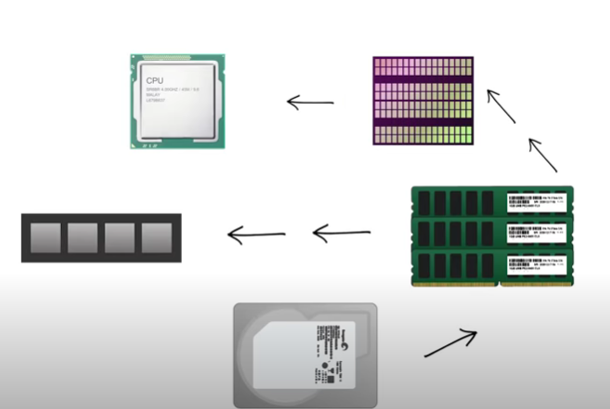
\includegraphics[width=1.00\textwidth]{imagen 2.PNG}
La imagen corresponde al video de  \cite{memoria}
\vspace{0.2cm}

Cada memoria del computador cumple con una función de acuerdo a sus capacidades, considerando que la memoria RAM es mucho más rápida que el disco  y  para que el procesador no se quede esperando la carga de datos, se utiliza la RAM. Pero si utilizamos solo esta memoria, el computador puede presentar intermitencias  en algunas ocasiones. Para esto se introdujo otro nivel de memoria llamado SRAM o memoria cache, este es un paso intermedio entre la RAM y el procesador; su principal función consiste en tener a la mano los procesos que se realizan de manera recurrente; por este motivo cuando  el procesador necesita buscar archivos se dirige en primer lugar a la memoria cache  y luego como segunda opción esta la memoria RAM, por último y en caso tal de no encontrar la información en las memorias anteriores este se dirige al disco duro y así se repite el proceso de intercambio de información entre ellos, hasta el momento en que el computador se apaga.


\section{¿Qué hace que una memoria sea más rápida que otra? ¿Por qué esto es importante?}

La velocidad de una memoria depende tanto de las especificaciones físicas como digitales, La memoria RAM y el disco duro se utilizan para almacenar información, pero sus funciones dentro de un PC son muy diferentes. En pocas palabras, la memoria RAM es una memoria de trabajo pero su capacidad de almacenamiento es inferior en comparación con el disco duro, el cual es una memoria de almacenamiento con grandes limitaciones en cuanto a su capacidad para encontrar información a tiempo; pero tanto el disco duro como la memoria RAM cumplen una función muy importante en el computador, puesto que es una complementacion mutua , cada una cumple con función especifica, tanto la memoria ROM,VRAM y cache son importante para asegurar el rendimiento de la velocidad en el computador; si pudiéramos tener una memoria que tenga  tanto velocidad como almacenamiento no sería necesario el uso de tantas memorias  para permitir un buen funcionamiento en el computador, posiblemente en el futuro esto sea posible pero actualmente son completamente indispensables para el PC.



\section{Conclusión} \label{conclulsion}
 \begin{itemize}
\item Cada memoria tiene una función especifica en el computador.
\item La gestión de los datos en un computador no son estaticos, estos siempre se encuentran en movimiento.

\item La falta de velocidad de una memoria se puede compensar con su capacidad de almacenamiento, por lo que algunas memorias pueden ser lentas pero fiables. otras pueden ser rapidas pero volatiles, y algunas mejoran gran parte del funcionamiento. En fin cada memoria tiene sus pros y sus contras, por ese motivo nuestro computador  utiliza tantas.

\end{itemize}

\newpage

\bibliographystyle{apacite}
\bibliography{sample.bib}


\end{document}


